\section{Aufbau und Durchführung}
\subsection{Aufbau}
Zur Durchführung des Versuches wird der in Abbildung \ref{fig:Aufbau} dargestellte Versuchsaufbau
verwendet.
\begin{figure}[H]
    \centering
    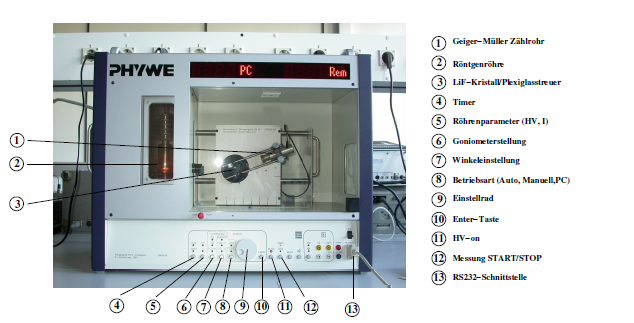
\includegraphics{Aufbau.png}
    \caption{Versuchsapparatur.}
    \label{fig:Aufbau}
\end{figure}
Die Apparatur enthält eine Cu-Röontgenröhre, einen LiF-Kristall und ein Geiger-Müller
Zählrohr und kann über das Programm measure vom Computer aus gesteuert werden.
So kann in dem Programm der Kristallwinkel, der Zählrohrwinkel und die Integrationszeit
eingestellt werden.
\subsection{Durchführung}
Für alle Messungen wird eine Beschleunigungsspannung von $U_B = 35\,\mathrm{kV}$ 
und ein Emissionsstrom um $I=1\,\mathrm{mA}$ verwendet.
\subsubsection{Überprüfung der Bragg-Bedingung}
Im ersten Versuchsteil wird die Bragg Bedingung überprüft. Der LiF-Kristall wird dafür
auf einen Winkel von $\theta=14°$ eingestellt. Und das Zählrohr misst die Intensität der
Röntgenstrahlung. Es wird von $\theta_\text{GM} =26°$ bis $\theta_\text{GM}=30°$ mit einem Winkelzuwachs von
$\Delta \theta_\text{GM} = 0,1°$ gemessen.
\subsubsection{Analyse eines Emissionsspektrums der Kupfer-Röntgenröhre}
Als nächstes wird das Emissionsspektrum der Cu-Röntgenröreh ausgemessen. Die Messungen
wird in $\Delta \theta = 0,1°$ Schritten aufgenommen mit einer Integrationszeit von $\Delta t =10\,\mathrm{s}$.
\subsubsection{Analyse der Absorptionsspektren}
Anschließend werden Absorptionsspekten verschiedener Materialien untersucht. Dazu
werden nacheinander 5 Absorber mit Kernladungszahlen zwischen 30 und 50 vor das
Geiger-Müller Zählrohr angebracht. Für die Winkel wird ein geeigneter Messbereich
gewählt. Die Messzeit ist $\Delta t=20\,\mathrm{s}$. 
\label{sec:Aufbau}
